\section{Factorial Hidden Markov Model (FHMM)}

An FHMM is an extension of the standard Hidden Markov Model (HMM) that allows for multiple independent hidden state sequences to influence the observed data.

The problem of interest is to infer the marginals of the hidden states, and the most probable sequence of hidden states, given a sequence of observations in a Factorial Hidden Markov Model (FHMM).

The problem involved making a junction tree out of the FHMM by triangulating it and then using the message passing algorithm to infer the marginals of the hidden states and the most probable sequence of hidden states given a sequence of observations.

\vspace{1cm}
\begin{center}
\begin{tikzpicture}[
    ->, >=Stealth, auto, node distance=3cm,
    state/.style={circle, draw, minimum size=0.8cm, font=\footnotesize},
    obs/.style={rectangle, draw, minimum size=1cm, font=\footnotesize},
    every edge/.style={draw, thick}
]

% Hidden states for Factor 1 (bottom of inverted triangle)
\node[state] (S1_1) at (0, 4) {$S_1^{(1)}$};
\node[state] (S1_2) at (4, 4) {$S_2^{(1)}$};
\node[state] (S1_3) at (8, 4) {$S_3^{(1)}$};

% Hidden states for Factor 2 (top-left of inverted triangle)
\node[state] (S2_1) at (-0.75, 5.5) {$S_1^{(2)}$};
\node[state] (S2_2) at (3.25, 5.5) {$S_2^{(2)}$};
\node[state] (S2_3) at (7.25, 5.5) {$S_3^{(2)}$};

% Hidden states for Factor 3 (top-right of inverted triangle)
\node[state] (S3_1) at (0.75, 5.5) {$S_1^{(3)}$};
\node[state] (S3_2) at (4.75, 5.5) {$S_2^{(3)}$};
\node[state] (S3_3) at (8.75, 5.5) {$S_3^{(3)}$};

% Observations (below the inverted triangle)
\node[obs] (O1) at (0, 2.5) {$O_1$};
\node[obs] (O2) at (4, 2.5) {$O_2$};
\node[obs] (O3) at (8, 2.5) {$O_3$};

% Transition edges for Factor 1 (more bent)
\path (S1_1) edge[bend left=30] (S1_2);
\path (S1_2) edge[bend left=30] (S1_3);

% Transition edges for Factor 2 (more bent)
\path (S2_1) edge[bend left=30] (S2_2);
\path (S2_2) edge[bend left=30] (S2_3);

% Transition edges for Factor 3 (more bent)
\path (S3_1) edge[bend left=30] (S3_2);
\path (S3_2) edge[bend left=30] (S3_3);

% Observation edges for t=1 (more bent)
\path (S1_1) edge (O1);
\path (S2_1) edge[bend right=50] (O1);
\path (S3_1) edge[bend left=50] (O1);

% Observation edges for t=2 (more bent)
\path (S1_2) edge (O2);
\path (S2_2) edge[bend right=50] (O2);
\path (S3_2) edge[bend left=50] (O2);

% Observation edges for t=3 (more bent)
\path (S1_3) edge (O3);
\path (S2_3) edge[bend right=50] (O3);
\path (S3_3) edge[bend left=50] (O3);

\end{tikzpicture}
\end{center}

The moralized graph looks like

\begin{center}
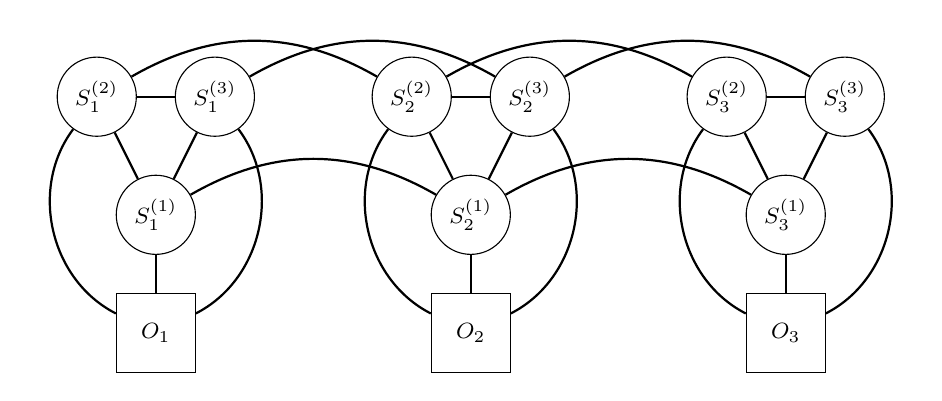
\begin{tikzpicture}[
    auto, node distance=3cm,
    state/.style={circle, draw, minimum size=0.8cm, font=\footnotesize},
    obs/.style={rectangle, draw, minimum size=1cm, font=\footnotesize},
    every edge/.style={draw, thick}
]

% Hidden states for Factor 1 (bottom of inverted triangle)
\node[state] (S1_1) at (0, 4) {$S_1^{(1)}$};
\node[state] (S1_2) at (4, 4) {$S_2^{(1)}$};
\node[state] (S1_3) at (8, 4) {$S_3^{(1)}$};

% Hidden states for Factor 2 (top-left of inverted triangle)
\node[state] (S2_1) at (-0.75, 5.5) {$S_1^{(2)}$};
\node[state] (S2_2) at (3.25, 5.5) {$S_2^{(2)}$};
\node[state] (S2_3) at (7.25, 5.5) {$S_3^{(2)}$};

% Hidden states for Factor 3 (top-right of inverted triangle)
\node[state] (S3_1) at (0.75, 5.5) {$S_1^{(3)}$};
\node[state] (S3_2) at (4.75, 5.5) {$S_2^{(3)}$};
\node[state] (S3_3) at (8.75, 5.5) {$S_3^{(3)}$};

% Observations (below the inverted triangle)
\node[obs] (O1) at (0, 2.5) {$O_1$};
\node[obs] (O2) at (4, 2.5) {$O_2$};
\node[obs] (O3) at (8, 2.5) {$O_3$};

% Transition edges for Factor 1 (undirected, curved)
\path (S1_1) edge[bend left=30] (S1_2);
\path (S1_2) edge[bend left=30] (S1_3);

\path (S1_1) edge (S2_1);
\path (S2_1) edge (S3_1);
\path (S3_1) edge (S1_1);

\path (S1_2) edge (S2_2);
\path (S2_2) edge (S3_2);
\path (S3_2) edge (S1_2);

\path (S1_3) edge (S2_3);
\path (S2_3) edge (S3_3);
\path (S3_3) edge (S1_3);

% Transition edges for Factor 2 (undirected, curved)
\path (S2_1) edge[bend left=30] (S2_2);
\path (S2_2) edge[bend left=30] (S2_3);

% Transition edges for Factor 3 (undirected, curved)
\path (S3_1) edge[bend left=30] (S3_2);
\path (S3_2) edge[bend left=30] (S3_3);

% Observation edges for t=1 (undirected, curved)
\path (S1_1) edge (O1);
\path (S2_1) edge[bend right=50] (O1);
\path (S3_1) edge[bend left=50] (O1);

% Observation edges for t=2 (undirected, curved)
\path (S1_2) edge (O2);
\path (S2_2) edge[bend right=50] (O2);
\path (S3_2) edge[bend left=50] (O2);

% Observation edges for t=3 (undirected, curved)
\path (S1_3) edge (O3);
\path (S2_3) edge[bend right=50] (O3);
\path (S3_3) edge[bend left=50] (O3);

\end{tikzpicture}
\end{center}

The junction tree made out of the cliques after triangulation is a chain as shown below:

\begin{center}
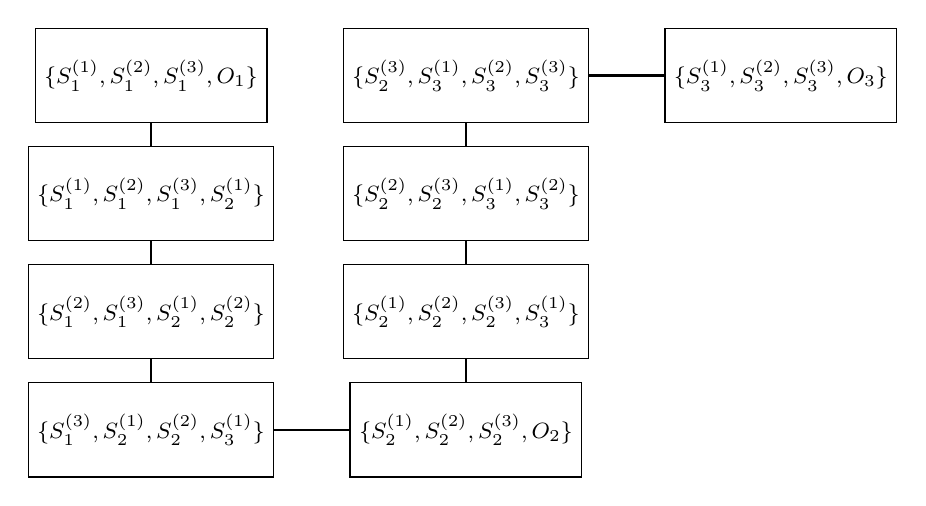
\begin{tikzpicture}[
    auto, node distance=4cm,
    clique/.style={rectangle, draw, minimum size=1.2cm, font=\footnotesize},
    every edge/.style={draw, thick}
]
% Cliques
\node[clique] (C1) at (0, 0) {$\{S_1^{(1)}, S_1^{(2)}, S_1^{(3)}, O_1\}$};
\node[clique] (C2) at (0, -1.5) {$\{S_1^{(1)}, S_1^{(2)}, S_1^{(3)}, S_2^{(1)}\}$};
\node[clique] (C3) at (0, -3) {$\{S_1^{(2)}, S_1^{(3)}, S_2^{(1)}, S_2^{(2)}\}$};
\node[clique] (C4) at (0, -4.5) {$\{S_1^{(3)}, S_2^{(1)}, S_2^{(2)}, S_3^{(1)}\}$};

\node[clique] (C5) at (4, -4.5) {$\{S_2^{(1)}, S_2^{(2)}, S_2^{(3)}, O_2\}$};
\node[clique] (C6) at (4, -3) {$\{S_2^{(1)}, S_2^{(2)}, S_2^{(3)}, S_3^{(1)}\}$};
\node[clique] (C7) at (4, -1.5) {$\{S_2^{(2)}, S_2^{(3)}, S_3^{(1)}, S_3^{(2)}\}$};
\node[clique] (C8) at (4, 0) {$\{S_2^{(3)}, S_3^{(1)}, S_3^{(2)}, S_3^{(3)}\}$};

\node[clique] (C9) at (8, 0) {$\{S_3^{(1)}, S_3^{(2)}, S_3^{(3)}, O_3\}$};
% Edges between cliques
\path (C1) edge (C2);
\path (C2) edge (C3);
\path (C3) edge (C4);
\path (C4) edge (C5);
\path (C5) edge (C6);
\path (C6) edge (C7);
\path (C7) edge (C8);
\path (C8) edge (C9);
\end{tikzpicture}
\end{center}

The message passing algorithm is now simple with just two passes, one from left to right and the other from right to left.

For including the prior of the observations, we merged the observations into the cliques by removing the observation nodes and considering the potentials over the cliques that include the observations.

For finding the z-value of the junction tree, the message passing algorithm runs over every clique for 
